\documentclass[DIV=15,
fleqn
numbers=noenddot,
headsepline,
captions=tableabove,twoside, openright]{scrreprt}
\usepackage{pgf,tikz}
\usepackage[utf8]{inputenc}
\usepackage[T1]{fontenc}
\usepackage[english]{babel}
\usepackage[intlimits,slantedGreeks]{kpfonts}
\usepackage[expansion=false]{microtype}
\usepackage{bm}
\usepackage[]{graphicx}
\usepackage{psfrag}\usepackage{amsmath}
\usepackage{amsfonts}
\usepackage{amssymb}
\usepackage{graphics}
\usepackage{color}
\usepackage{colortbl, hhline}
\usepackage{subfigure}
\usepackage{float}
\usepackage{url}
\usepackage{upgreek}
\usepackage{multicol,caption}
\usepackage[titletoc]{appendix}
\usepackage{mathtools}
\usepackage{amsmath}
\usepackage{calc}
\usepackage{epstopdf}
\usepackage{units}
\usepackage{tabularx}
\usepackage{booktabs}
\usepackage{longtable}
\usepackage{listings}
\usepackage[automark]{scrpage2}
\usepackage{babelbib}
\usepackage{tikz}
\usetikzlibrary{shapes,arrows,positioning,decorations.pathreplacing,calc}
\tikzset{cross/.style={cross out, draw=black, minimum size=2*(#1-\pgflinewidth), inner sep=0pt, outer sep=0pt},
	%default radius will be 1pt. 
	cross/.default={0.1 cm}}
%-----------------NEW PACKAGES from October2017--------%
\usepackage[]{datetime2}
\usepackage{enumitem}
\setlist[description]{leftmargin=2cm,labelindent=2cm}
\usepackage{schemabloc}
\usepackage{acro}
\DeclareAcronym{mimo}{
	short = MIMO,
	long = Multiple-Input Multiple-Output}
\usepackage{cleveref}
\DeclareAcronym{fmcw}{
	short = FMCW,
	long = Frequency-Modulated Continuous-Wave}
\DeclareAcronym{if}{
	short = IF , long =
	intermediate frequency }
\DeclareAcronym{fft}{
	short = FFT , long = Fast Fourier Transform }
\DeclareAcronym{mtt}{
	short =MTT,
    long = Multi-Target Tracking }
\DeclareAcronym{lti}{
	short = LTI , long = Linear Time Invariant}
\DeclareAcronym{nn}{
	short = NN , long = nearest-neighbor}
\DeclareAcronym{dbscan}{
	short = DBSCAN , long = density-based spatial clustering of applicatios with noise}
\DeclareAcronym{dbd}{
	short =DBD , long =density-based-decomposition}
%ausprobieren
\setcounter{secnumdepth}{2}
\setcounter{tocdepth}{2}
%ausprobieren ende
\usepackage{slashbox}
\newcolumntype{K}[1]{>{\centering\arraybackslash}p{#1}}


\pagestyle{scrplain}
\clearscrheadfoot
\ihead{}
\chead{}
\ohead{}
\ifoot{}
\cfoot[\pagemark]{\pagemark}
\ofoot{}

	

\setkomafont{disposition}     {\normalfont\bfseries}
\setkomafont{descriptionlabel}{\normalfont\bfseries}
\setkomafont{pagehead}        {\normalfont}
\setkomafont{caption}         {\normalfont\small}
\setkomafont{captionlabel}    {\normalfont\small\bfseries}
\setcapindent{0em}

\setcounter{secnumdepth}{3}
\setcounter{tocdepth}{3}

\setcounter{topnumber}           {1}
\setcounter{bottomnumber}        {1}
\renewcommand{\floatpagefraction}{0.8}
\renewcommand{\topfraction}      {0.8}
\renewcommand{\bottomfraction}   {0.5}
\renewcommand{\textfraction}     {0.15}
\makeatletter
\setlength{\@fptop}{0pt}
\makeatother
%--------------------Command definitions--------------%
\newcommand*{\mj}   {\mathrm{j}}
\newcommand*{\me}   {\mathrm{e}}
\newcommand*{\Div}  {\operatorname{div}}
\newcommand*{\Rot}  {\operatorname{rot}}
\newcommand*{\Grad} {\operatorname{grad}}
\renewcommand*{\Re} {\operatorname{Re}}
\renewcommand*{\Im} {\operatorname{Im}}
\renewcommand{\Re}  {\operatorname{Re}}
\renewcommand{\Im}  {\operatorname{Im}}
\renewcommand{\vec}   [1]{\bm{#1}}
\renewcommand{\matrix}[1]{\mathbf{#1}}
\newcommand* {\snr} {\mathrm{SNR}}
\newcommand{\Iog}  {\operatorname{log}}
\newcommand*\diff{\mathop{}\!\mathrm{d}}
\newcommand*\Diff[1]{\mathop{}\!\mathrm{d^#1}}
\newcommand*{\Expc}{\mathbf{E}}
\newcommand*{\diag}  {\operatorname{diag}}
%\newcommand*{\max}  {\operatorname{max}}
\addto\captionsenglish{%
	\renewcommand{\figurename}{Figure}%
}


\AtBeginDocument{\bbbbaddto{english} {btxifchangecaseoff}}
\bibliographystyle{unsrt}
\usepackage{titlesec}


\usetikzlibrary{arrows}


%------------------Date Settings------------------------%
\DTMsetdatestyle{ddmmyyyy}

\begin{document}
%---------------------COVER------------------------------%
\input{cover/cover}
%-------------------FIRST PAGES-------------------------%

\pagenumbering{Roman}
\chapter*{Sperrvermerk}

\chapter*{Declaration of Authorship}
\chapter*{}
\vspace*{8cm}
\thispagestyle{empty}
%------------------DEDICATION--------------------------------%
\input{cover/Dedication}
%--------------------Contents--------------------------------%
\tableofcontents	
%***********************************************
%INTRODUCTION
%***********************************************
\chapter{Introduction}
	\pagenumbering{arabic}
	\pagestyle{scrheadings}
	\clearscrheadfoot
	\ihead{\headmark}
	\ohead{\pagemark}
\begin{figure}[h!]
	\centering
	
\begin{tikzpicture}
% Reference Grid
\draw[gray,very thin] (0,0) grid (10,4); 

\end{tikzpicture}
	\caption{Block Diagram of the whole process}
	\label{fig:intro}
\end{figure} 
\chapter{Radar Fundamentals}\label{ch:basics}
\begin{figure}[h!]
	\centering
	
\begin{tikzpicture}
% Reference Grid
\draw[gray,very thin] (0,0) grid (10,4); 

\end{tikzpicture}
	\caption{Block Diagram of the whole process}
	\label{fig:intro}
\end{figure} 
\section{Radar Definitions}\label{bs:definitions}
 Range
\begin{equation}
	R = \frac{c_0\Delta t}{2}
\end{equation}
Pulse repetition interval (PRI)
\begin{equation}
	f_r = \frac{1}{T}
\end{equation}
Unambiguous range  $R_u$
\begin{figure}
	\centering
	
\begin{tikzpicture}
% Reference Grid
\draw[gray,very thin] (0,0) grid (10,4); 

\end{tikzpicture}
	\caption{Illustrating the unambiguous range}
\end{figure} 
 \section{MIMO Array}\label{bs:MIMO}
 For the estimation of the azimuth and elevation of a target's position, the phase array radar has been a popular choice during the past decades. This technique employs a series of antennas to transmit and receive the electromagnetic waveform before mentioned. Here, the phase of each element in the group of transmitted is adjusted for the radar to be able to suppress the response from specific directions and thus, "scan" a specific direction. The angular resolution of this method, however, strongly depends on the number of elements in the antenna array. An attractive alternative to the simple phase array is its combination with the \ac{mimo} concept \cite{fishler_mimo_2004}. 

As the name implies, a \ac{mimo} radar consists of multiple transmit (TX) antennas and receive (RX) antennas. $M_t$ transmit and $M_r$ receive elements are assumed. The difference from the phase array radar is that the signals transmitted by each of the TX elements are diversified, leading to $M_t\times M_r$ propagation channels. This, with only $M_t + M_r$ antenna elements. With this concept, a higher performance with a substantially lower cost can be achieved, which is why the \ac{mimo} array has been chosen for the purpose of this thesis. 

Several methods to the define the diversity of the TX channels have been proposed, these include frequency division multiplexing, spatial coding, orthogonal waveforms and time division multiplexing. The latter has been chosen and implemented as presented in \cite{huang_fmcw_2011}. As the name indicates and as presented in \cref{fig:tdm}, the concept time division multiplexing consists in switching the transmit antenna at each consecutive pulse. Hereby, one is able to differentiate at the receiver from which TX element is the signal coming simply by looking at the time of reception, which is important for the estimation of the azimuth profile (\cref{bs:azimuth}).


\begin{figure}[h!]
	\centering
	
\begin{tikzpicture}
% Reference Grid
\draw[gray,very thin] (0,0) grid (10,4); 

\end{tikzpicture}
	\caption{Time division multiplexing for \Ac{mimo}-radar.}
	\label{fig:tdm}
\end{figure} 


A further design concern is the array manifold. Different array forms can be found in literature, where the most common are the uniform linear array (ULA) and the uniform circular array (UCA) \cite{zhang_blind_2009}, which are depicted in \cref{fig:ula,fig:uca}. As the name indicates, this manifolds consists of equidistant antenna elements in either linear or circular form. The MIMO-radar chosen here consists in 2 TX and 4 RX array resulting in 8 virtual channels.

\begin{figure}[h!]
	\centering
	\begin{minipage}{.5\textwidth}
		\centering
		
\begin{tikzpicture}
% Reference Grid
\draw[gray,very thin] (0,0) grid (7,5); 

\end{tikzpicture}
		\captionof{figure}{Uniform Linear Array (ULA).}
		\label{fig:ula}
	\end{minipage}%
	\begin{minipage}{.5\textwidth}
		\centering
		
\begin{tikzpicture}
% Reference Grid
\draw[gray,very thin] (0,0) grid (7,5); 

\end{tikzpicture}
		\captionof{figure}{Uniform Circular Array (UCA).}
		\label{fig:uca}
	\end{minipage}
\end{figure}

If the far-field condition is satisfied, the \Ac{mimo}-configuration can be modeled as an ULA of  $M_t\times M_r$ virtual antennas. Given the position of the TX-elements $x_i^{Tx}$ and RX-elements $x_j^{Rx}$ the virtual ULA is modeled by antenna elements at 

\begin{equation}
\vec{x_{ij}} = (\vec{x}_i^{Tx}+\vec{x}_j^{Rx})/2\\,
\end{equation}
for $i = 1,...,M_t$ and $j = 1,...,M_r$. Presented in \cref{fig:mimo_array} is a \Ac{mimo}-setup with its corresponding virtual elements. Note that for this work the TX and RX elements are aligned in the vertical axis. This has been ignored here for better illustration. 

\begin{figure}[h]
	\centering
	For the estimation of the azimuth and elevation of a target's position, the phase array radar has been a popular choice during the past decades. This technique employs a series of antennas to transmit and receive the electromagnetic waveform before mentioned. Here, the phase of each element in the group of transmitted is adjusted for the radar to be able to suppress the response from specific directions and thus, "scan" a specific direction. The angular resolution of this method, however, strongly depends on the number of elements in the antenna array. An attractive alternative to the simple phase array is its combination with the \ac{mimo} concept \cite{fishler_mimo_2004}. 

As the name implies, a \ac{mimo} radar consists of multiple transmit (TX) antennas and receive (RX) antennas. $M_t$ transmit and $M_r$ receive elements are assumed. The difference from the phase array radar is that the signals transmitted by each of the TX elements are diversified, leading to $M_t\times M_r$ propagation channels. This, with only $M_t + M_r$ antenna elements. With this concept, a higher performance with a substantially lower cost can be achieved, which is why the \ac{mimo} array has been chosen for the purpose of this thesis. 

Several methods to the define the diversity of the TX channels have been proposed, these include frequency division multiplexing, spatial coding, orthogonal waveforms and time division multiplexing. The latter has been chosen and implemented as presented in \cite{huang_fmcw_2011}. As the name indicates and as presented in \cref{fig:tdm}, the concept time division multiplexing consists in switching the transmit antenna at each consecutive pulse. Hereby, one is able to differentiate at the receiver from which TX element is the signal coming simply by looking at the time of reception, which is important for the estimation of the azimuth profile (\cref{bs:azimuth}).


\begin{figure}[h!]
	\centering
	
\begin{tikzpicture}
% Reference Grid
\draw[gray,very thin] (0,0) grid (10,4); 

\end{tikzpicture}
	\caption{Time division multiplexing for \Ac{mimo}-radar.}
	\label{fig:tdm}
\end{figure} 


A further design concern is the array manifold. Different array forms can be found in literature, where the most common are the uniform linear array (ULA) and the uniform circular array (UCA) \cite{zhang_blind_2009}, which are depicted in \cref{fig:ula,fig:uca}. As the name indicates, this manifolds consists of equidistant antenna elements in either linear or circular form. The MIMO-radar chosen here consists in 2 TX and 4 RX array resulting in 8 virtual channels.

\begin{figure}[h!]
	\centering
	\begin{minipage}{.5\textwidth}
		\centering
		
\begin{tikzpicture}
% Reference Grid
\draw[gray,very thin] (0,0) grid (7,5); 

\end{tikzpicture}
		\captionof{figure}{Uniform Linear Array (ULA).}
		\label{fig:ula}
	\end{minipage}%
	\begin{minipage}{.5\textwidth}
		\centering
		
\begin{tikzpicture}
% Reference Grid
\draw[gray,very thin] (0,0) grid (7,5); 

\end{tikzpicture}
		\captionof{figure}{Uniform Circular Array (UCA).}
		\label{fig:uca}
	\end{minipage}
\end{figure}

If the far-field condition is satisfied, the \Ac{mimo}-configuration can be modeled as an ULA of  $M_t\times M_r$ virtual antennas. Given the position of the TX-elements $x_i^{Tx}$ and RX-elements $x_j^{Rx}$ the virtual ULA is modeled by antenna elements at 

\begin{equation}
\vec{x_{ij}} = (\vec{x}_i^{Tx}+\vec{x}_j^{Rx})/2\\,
\end{equation}
for $i = 1,...,M_t$ and $j = 1,...,M_r$. Presented in \cref{fig:mimo_array} is a \Ac{mimo}-setup with its corresponding virtual elements. Note that for this work the TX and RX elements are aligned in the vertical axis. This has been ignored here for better illustration. 

\begin{figure}[h]
	\centering
	For the estimation of the azimuth and elevation of a target's position, the phase array radar has been a popular choice during the past decades. This technique employs a series of antennas to transmit and receive the electromagnetic waveform before mentioned. Here, the phase of each element in the group of transmitted is adjusted for the radar to be able to suppress the response from specific directions and thus, "scan" a specific direction. The angular resolution of this method, however, strongly depends on the number of elements in the antenna array. An attractive alternative to the simple phase array is its combination with the \ac{mimo} concept \cite{fishler_mimo_2004}. 

As the name implies, a \ac{mimo} radar consists of multiple transmit (TX) antennas and receive (RX) antennas. $M_t$ transmit and $M_r$ receive elements are assumed. The difference from the phase array radar is that the signals transmitted by each of the TX elements are diversified, leading to $M_t\times M_r$ propagation channels. This, with only $M_t + M_r$ antenna elements. With this concept, a higher performance with a substantially lower cost can be achieved, which is why the \ac{mimo} array has been chosen for the purpose of this thesis. 

Several methods to the define the diversity of the TX channels have been proposed, these include frequency division multiplexing, spatial coding, orthogonal waveforms and time division multiplexing. The latter has been chosen and implemented as presented in \cite{huang_fmcw_2011}. As the name indicates and as presented in \cref{fig:tdm}, the concept time division multiplexing consists in switching the transmit antenna at each consecutive pulse. Hereby, one is able to differentiate at the receiver from which TX element is the signal coming simply by looking at the time of reception, which is important for the estimation of the azimuth profile (\cref{bs:azimuth}).


\begin{figure}[h!]
	\centering
	\input{fundamentals_figs/blank.tex}
	\caption{Time division multiplexing for \Ac{mimo}-radar.}
	\label{fig:tdm}
\end{figure} 


A further design concern is the array manifold. Different array forms can be found in literature, where the most common are the uniform linear array (ULA) and the uniform circular array (UCA) \cite{zhang_blind_2009}, which are depicted in \cref{fig:ula,fig:uca}. As the name indicates, this manifolds consists of equidistant antenna elements in either linear or circular form. The MIMO-radar chosen here consists in 2 TX and 4 RX array resulting in 8 virtual channels.

\begin{figure}[h!]
	\centering
	\begin{minipage}{.5\textwidth}
		\centering
		\input{fundamentals_figs/blank2.tex}
		\captionof{figure}{Uniform Linear Array (ULA).}
		\label{fig:ula}
	\end{minipage}%
	\begin{minipage}{.5\textwidth}
		\centering
		\input{fundamentals_figs/blank2.tex}
		\captionof{figure}{Uniform Circular Array (UCA).}
		\label{fig:uca}
	\end{minipage}
\end{figure}

If the far-field condition is satisfied, the \Ac{mimo}-configuration can be modeled as an ULA of  $M_t\times M_r$ virtual antennas. Given the position of the TX-elements $x_i^{Tx}$ and RX-elements $x_j^{Rx}$ the virtual ULA is modeled by antenna elements at 

\begin{equation}
\vec{x_{ij}} = (\vec{x}_i^{Tx}+\vec{x}_j^{Rx})/2\\,
\end{equation}
for $i = 1,...,M_t$ and $j = 1,...,M_r$. Presented in \cref{fig:mimo_array} is a \Ac{mimo}-setup with its corresponding virtual elements. Note that for this work the TX and RX elements are aligned in the vertical axis. This has been ignored here for better illustration. 

\begin{figure}[h]
	\centering
	\input{fundamentals_figs/mimo.tex}
	\caption{\ac{mimo}-array}
		\label{fig:mimo_array}
\end{figure} 
 
 Under the described conditions the signal propagation path from a given TX element to a scatterer at point $\vec{p}$, plus the reflection path back to an RX element can be approximated as
 \begin{equation}
 	P_{ij}(p) = |\vec{p}-\vec{x}_i^{Tx}| + |\vec{p}-\vec{x}_j^{Rx}| \approx 2|\vec{p}-\vec{x}_{ij}| \\.
 \end{equation}
	\caption{\ac{mimo}-array}
		\label{fig:mimo_array}
\end{figure} 
 
 Under the described conditions the signal propagation path from a given TX element to a scatterer at point $\vec{p}$, plus the reflection path back to an RX element can be approximated as
 \begin{equation}
 	P_{ij}(p) = |\vec{p}-\vec{x}_i^{Tx}| + |\vec{p}-\vec{x}_j^{Rx}| \approx 2|\vec{p}-\vec{x}_{ij}| \\.
 \end{equation}
	\caption{\ac{mimo}-array}
		\label{fig:mimo_array}
\end{figure} 
 
 Under the described conditions the signal propagation path from a given TX element to a scatterer at point $\vec{p}$, plus the reflection path back to an RX element can be approximated as
 \begin{equation}
 	P_{ij}(p) = |\vec{p}-\vec{x}_i^{Tx}| + |\vec{p}-\vec{x}_j^{Rx}| \approx 2|\vec{p}-\vec{x}_{ij}| \\.
 \end{equation}
\section{Signal Model}\label{bs:signal}
For the following analyses a \Ac{fmcw} Radar is taken into consideration. The TX array elements transmit a \Ac{fmcw} chirp signal, that can be modeled in as
\begin{equation}
	s_T(t) = \exp[\mj(2\pi f_ct+\pi kt^2)]\\,
\end{equation}
for $-T_c/2 \leq t \leq T_c/2$, where $T_c$ is the chirp duration, $f_c$ the carrier frequency and the chirp rate $k$ is defined by
\begin{equation}
	k = \pm B/T_c\\.
\end{equation}
Under far-field condition, the return delay between a virtual element at $x_{ij}$ and a scatterer is given by
\begin{equation}
	\Delta t_{ij} = \frac{2R}{c_0} + \frac{2x_{ij}\sin\theta}{c_0}\\,
\end{equation}
where $R$ and $\theta$ describe the location of the scatterer, $R$ being the rang and $\theta$ the angle with respect to boresight. The received signal 
\begin{equation}
	s_R^{ij}(t) = As_t(t-\Delta t_{ij})
\end{equation}
After the signal is received, it is down-converted by multiplying it with a replica of the transmitted signal. After low-pass filtering, the processed signal can be modeled as 
\begin{equation}
	u_{ij}(t) = s_R^{ij}s_T(t) = A\exp[\mj(2\pi k \Delta t_{ij}t-\pi k\Delta  t_{ij}^2 + 2\pi f_c \Delta t_{ij})]
\end{equation}
The sampled form of the \ac{if} signal given $N$ samples can be expressed as
\begin{equation}
	u_{ij}[n] = A\exp[\mj(\phi+2\pi\Psi_R n)]\\,
\end{equation}
with $\Psi_R = k\Delta t_{ij}\frac{T_c}{N} $,the normalized frequency containing the range information and $\phi = -\pi k\Delta  t_{ij}^2 + 2\pi f_c \Delta t_{ij} $ contains the phase information. This expression can be generalized to \ac{mimo} radar, with $M$ targets either static or dynamic, for the $k$-th observation interval by
\begin{equation}\label{eq:signal}
	u_{k}[n,n_C,n_A] = \sum_{m=0}^{M}A_m\exp[\mj2\pi(\phi_m+\Psi_{R,m}n+\Psi_{D,m}n_C+\Psi_{\theta,m}n_A)] + w[n,n_C,n_A]
\end{equation}
where $\Psi_D = \frac{2T_cf_0}{c_0}v_R$ and $\Psi_\theta =\sin(\theta)/2 $ are the normalized frequencies containing the information about range-rate and azimuth. Moreover, $w[n,n_C,n_A]$ is the present additive white Gaussian measurement noise. The parameters $n$, $n_C$ and $n_A$ represent which, sample chirp and antenna is being taken into account. Please note that $\phi_m$ does not correspond to $\phi$.

The information collected from \cref{eq:signal} is usually arrange into a three-dimensional data cube as presented in \cref{fig:datacube}. Here the dimensions correspond to sample number, transmit-receive channel and chirp number. 

\begin{figure}[h]
	\centering
	
\begin{tikzpicture}
% Reference Grid
\draw[gray,very thin] (0,0) grid (10,4); 

\end{tikzpicture}
	\caption{Data Cube}
	\label{fig:datacube}
\end{figure} 

In order to estimate the spectrum of the received signal and so to determine the unknown parameters $R$, $v_R$ and $\theta$ for a given target, usually a three-dimensional \ac{fft} is applied to de \Ac{if} signal
\begin{multline}
\hat{P}_k(\Psi_R,\Psi_D\Psi_\theta) = \sum_{n}\sum_{n_C}\sum_{n_A} a_R[n] a_D[n_C] a_\theta[n_A]u_k[n,n_A,n_C]\\
\times\exp(-\mj2\pi\Psi_Rn)\exp(-\mj2\pi\Psi_Dn_C)\exp(-\mj2\pi\Psi_\theta n_A) \rlap{,}
\end{multline}
however, this usually results in a bad estimation for the azimuth range. Specifics of the signal processing will be described in the following sections. 
\section{Range and Range-Rate Estimation}\label{bs:range}
The estimation of the range and the range rate can be done by using a two-dimensional fft in the first and third dimension of the data cube.

\begin{equation}
\hat{P}_k(\Psi_R,\Psi_D) = \sum_{n}\sum_{n_C} a_R[n] a_D[n_C] u_k[n,n_A,n_C]\times\exp(-\mj2\pi\Psi_Rn)\exp(-\mj2\pi\Psi_Dn_C) \rlap{,}
\end{equation}

That's all for now, but what about Space- Adaptive Time Processing? WORK IN PROGRESS

\begin{figure}[h]
	\centering
	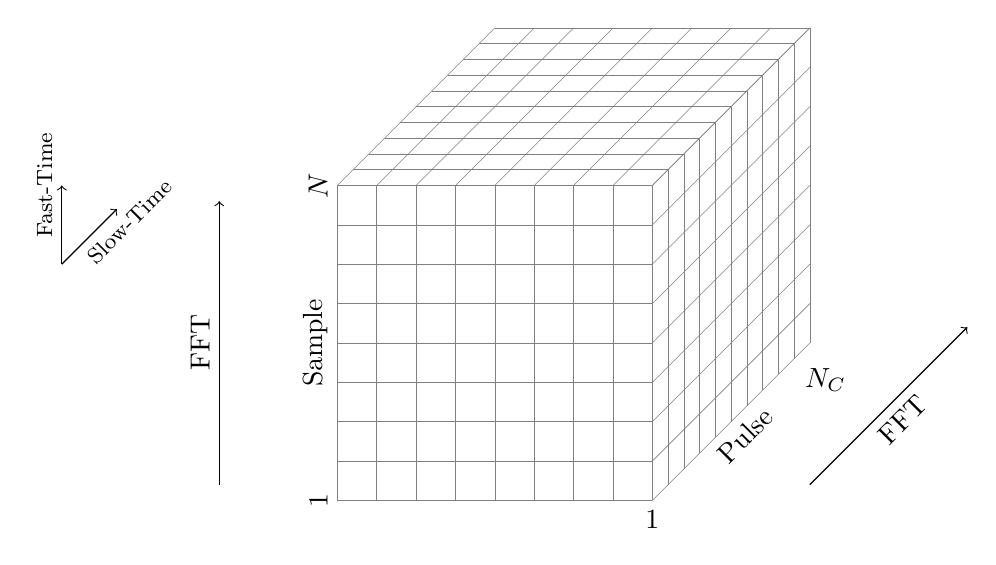
\begin{tikzpicture}
% Reference Grid

   \tikzstyle{virt} = [draw, shape=rectangle, minimum height=0.1cm, minimum width=0.1cm, node distance=0.0005cm and 0.0005cm, line width=1pt, fill = black]
   
\draw[gray,very thin,step = 0.5] (7.49,0) grid (11.5,4); 
%\draw[gray,very thin,step = 0.5] (9.49,2) grid (13.5,6); 

\foreach \x in {7.5,8,...,11.5}
    \draw[gray,very thin] (\x,4)--($(\x,4)+(2,2)$); 
    
\foreach \x in {0,0.5,...,4}
    \draw[gray,very thin] (11.5,\x)--($(11.5,\x)+(2,2)$); 
    
\foreach \x in {0.1,0.2,...,1}
    \draw[gray,very thin] ($(11.5,4)!\x!(13.5,6)$)-- ($(11.5,0)!\x!(13.5,2)$); 
    
\foreach \x in {0.1,0.2,...,1}
\draw[gray,very thin] ($(11.5,4)!\x!(13.5,6)$)-- ($(7.5,4)!\x!(9.5,6)$);     


\node at (7.5,2) [anchor = south,rotate = 90] {Sample}; 
\node at (12.5,1) [anchor = north, rotate = 45, align = center] {Pulse}; 
\node at (7.5,0) [anchor = south,rotate = 90]{$1$}; 
\node at (7.5,4) [anchor = south, rotate=90] {$N$}; 
\node at (11.5,0) [anchor = north, rotate = 0]{1}; 
\node at (13.7,1.8) [anchor = north]{$N_C$}; 

\draw[->] (4,3)-- (4,4)node[anchor=south,rotate = 90] {\footnotesize Fast-Time}; 
\draw[->] (4,3)-- (4.7,3.7)node[anchor=north,rotate = 45] {\footnotesize Slow-Time}; 
\draw[->] (6,0.2)--(6,3.8) ; 
\node at (6,2)[anchor = south,rotate =90](){FFT}; 
\draw[->] (13.5,0.2)--(15.5,2.2); 
\node at (14.5,1.2)[anchor = north,rotate =45](){FFT}; 
\end{tikzpicture}
	\caption{CHANGE TO ILLUSTRATE DATA PROCESSING }
	\label{fig:datacube2}
\end{figure} 



\section{Azimuth Estimation}\label{bs:azimuth}
Further definitions, for an antenna array the measured vector at time step $t$ can be obtained by
\begin{equation}
	\vec{x}(t) = \vec{a}(\theta){s}(t)\\,
\end{equation}

where ${s}(t)$ is the received waveform, $\vec{x}(t)$ the value observed at the virtual elements and $\vec{a}(\theta)$ are called the steering vectors. The vector $\vec{x}(t)$ thus, can be expressed by 
\begin{equation}
	\vec{x}(t) = \begin{bmatrix}
	x_1(t) & x_2(t) &... & x_L(t)
	\end{bmatrix}^T
\end{equation}
where $L$ is the number of virtual elements. The steering vector depends on the arrangement of the radar array, for ULA it can be written as
\begin{equation}
	\vec{a}_{ULA}(\theta) = \begin{bmatrix}
	1 & e^{-\mj kd cos \theta} & ... & e^{-\mj(L-1) kd cos \theta} 
	\end{bmatrix} 
\end{equation}
where $d$ is the separation between virtual elements. Assuming that $M$ point scatterers are present in the measurement space, the received signal results in
\begin{equation}
	\vec{x}(t) = \sum_{m=1}^{M}\vec{a}(\theta_m)s_m(t)\\,
\end{equation}
which can be expressed by the matrix notation 
\begin{equation}
	\vec{x}(t) = \matrix{A}(\theta) \vec{s}(t) + \vec{n}(t)\\,
\end{equation}
where 
\begin{equation}
	\matrix{A}(\theta) = \begin{bmatrix}
	\vec{a}(\theta_1) & ... & \vec{a}(\theta_M)
	\end{bmatrix}
\end{equation}
and
\begin{equation}
\vec{s}(t) = \begin{bmatrix}
s_1(t) & ... & s_M(t)
\end{bmatrix}^T
\end{equation}
and $\vec{n}(t)$ is additive white Gaussian noise.  We further define the spatial covariance matrix as
\begin{equation}
\matrix{R} = \Expc\left\{\vec{x}(t)\vec{x}^H(t) \right\} = \matrix{A}\Expc\left\{\vec{s}(t)\vec{s}^H(t)\right\}+ \Expc \left\{\vec{n}(t)\vec{n}^H (t)\right\}
\end{equation}
where we further define 
\begin{equation}
\Expc\left\{\vec{s}(t)\vec{s}^H(t)\right\} = \matrix{P}\\.
\end{equation}
and
\begin{equation}
\Expc\left\{\vec{n}(t)\vec{n}^H(t)\right\} = \sigma ^2 \vec{I}\\.
\end{equation}
The $\matrix{R}$ can then be decomposed in to
\begin{equation}
\matrix{R} = \matrix{A}\matrix{P}\matrix{A}^H+\sigma^2\matrix{I} = \matrix{U}\matrix{\Lambda}\matrix{U}\\.
\end{equation}
where $\matrix{U}$ is unitary and $\matrix{\Lambda} = \diag\left\{\lambda_1,\lambda_2,...,\lambda_L\right\}$ contains the eigenvalues ordered such as $\lambda_1 \geq \lambda_2 \geq ... \geq \lambda_L$
A further partition is made
\begin{equation}
	\matrix{R}  = \matrix{U}_s\matrix{\Lambda}_s\matrix{U}_s^H + \matrix{U}_n\matrix{\Lambda}_n\matrix{U}_n^H
\end{equation}
and the projectors are defined
\begin{equation}
\matrix{\Pi} =  \matrix{U}_s\matrix{U}_s^H = \matrix{A}(\matrix{A}^H\matrix{A})^{-1}\matrix{A}^H
\end{equation}
\begin{equation}
\matrix{\Pi}^\bot =  \matrix{U}_n\matrix{U}_n^H = \matrix{I}- \matrix{A}(\matrix{A}^H\matrix{A})^{-1}\matrix{A}^H
\end{equation}
\subsection{Conventional Beamforming}
Problem of maximizing the output power, formulation 

\begin{equation}
	\max_{\vec{w}} \Expc\left\{\vec{w}^H\vec{x}(t)\vec{x}^H(t)\vec{w}\right\}  = \max_{\vec{w}}\left\{\Expc|s(t)|^2|\vec{w}^H\vec{a}(\theta)|^2+\sigma^2|\vec{w}|^2\right\}\\,
\end{equation}

the solution is

\begin{equation}
 \vec{w}_{BF} = \frac{\vec{a}(\theta)}{\sqrt{\vec{a}^H(\theta)\vec{a}(\theta)}}
\end{equation}

so that the spatial spectrum can be expressed as
\begin{equation}
	P_{BF}(\theta) \frac{\vec{a}^H(\theta)\matrix{R}\vec{a}(\theta)}{\vec{a}^H(\theta)\vec{a}(\theta)}
\end{equation}

\begin{figure}[h!]
	\centering
	
\begin{tikzpicture}
% Reference Grid
\draw[gray,very thin] (0,0) grid (10,4); 

\end{tikzpicture}
	\caption{We do need some kind of real result.}
\end{figure} 

\subsection{The MUSIC-algorithm}
Based on the previous decomposition, the MUSIC algorithm takes advantage of the fact that the eigenvector in $\matrix{U}_n$ are orthogonal to the steering matrix $\matrix{A}$, i.e
\begin{equation}
	\matrix{U}_n^H\vec{a}(\theta) = 0\\, \quad \theta \in \left\{\theta_1,...,\theta_M\right\}
\end{equation}



The MUSIC "spatial spectrum" is defined as 

\begin{equation}
	P_M (\theta) = \frac{\vec{a}^H(\theta)\vec{a}(\theta)}{\vec{a}^H(\theta)\matrix{\Pi}^\bot\vec{a}(\theta)}
\end{equation}

\begin{figure}[h!]
	\centering
	
\begin{tikzpicture}
% Reference Grid
\draw[gray,very thin] (0,0) grid (10,4); 

\end{tikzpicture}
	\caption{We do need some kind of another real result.}
\end{figure} 

\chapter{Clustering}\label{ch:cluster}
Note: At the moment it is not clear whether other clustering algorithms which are not density-based decompositions will be considered. 
\section{Density-Based Clustering}\label{cs:Density}
Density-based clustering algorithms have been developed in the context of data mining in big data bases and knowledge discovery. For radar applications, density-based clustering is of advantage since it is very efficient in a dynamic environment where insertions and deletions are present. Furthermore, no cluster-prototype has to be specified, i.e. the clusters can be of arbitrary shape. Last but not least, the number of clusters does not have to be known in advance, which is a disadvantage that most clustering algorithms present which make them unsuitable for radar-applications. 

In \cref{cs:Def} some mathematical definitions that describe the way density-based clustering works are presented. Furthermore, \cref{cs:dbscan} presents the \ac{dbscan} algorithm.
\subsection{Definitions}\label{cs:Def}
The key idea of density-based clustering is that for most points of a cluster, the $\varepsilon$-neighborhood for some $\varepsilon > 0$, has to contain at least a minimum numbber of points. In other words, the neighborhood has to exceed a density-threshold to be considered a cluster. 

We define a distance-based $\varepsilon$-neighborhood  $N_\varepsilon$ of an object $o$  on a set of points $D$ by
\begin{equation}
	N_\varepsilon (o) = \{ o'\in D| |o-o'|\leq \varepsilon\}
\end{equation}
Furthermore, an object $p \in D$ is called \textit{directly density-reachable} from an object $q \in D$ if
\begin{enumerate}
	\item $p \in N_\varepsilon(q)$
	\item $size(N_\varepsilon(q))> MinPts$
\end{enumerate}
where $size()$ returns the number of points in an $\varepsilon$-neighborhood and $MinPts$ is the threshold that it has to meet to be considered a cluster. Morever, the object $p\in D$ is called \textit{density-reachable} from $q \in D$, if there is a chain of objects $p_1$,..., $p_n$, with $p_1 = q$ and $p_n =p$ such that for all $i =1$,..,$n-1$: $p_{i+1}$ is directly density-reachable o $p_{i}$. These definitions are illustrated in \cref{fig:density}

\begin{figure}[h]
	\centering
	
\begin{tikzpicture}
% Reference Grid
\draw[gray,very thin] (0,0) grid (10,4); 

\end{tikzpicture}
	\caption{Density-reachable example}
	\label{fig:density}
\end{figure} 

Finally, an object $p$ is density connected to an object $q$ if there exist an object $o$ such that both $p$ and $q$ are density-reachable from $o$, such as shown in \cref{fig:densityconn}.Note that all these properties are dependent on $\varepsilon$ and $MinPts$. In literature, for instance, it would be said that an object is density connected to another object with respect to $\varepsilon$ and $MinPts$, however this statement has been omitted since it is implied. 
\begin{figure}[h!]
	\centering
	
\begin{tikzpicture}
% Reference Grid
\draw[gray,very thin] (0,0) grid (10,4); 

\end{tikzpicture}
	\caption{Density-reachable example}
	\label{fig:densityconn}
\end{figure} 

With the previous definitions, one can now define the concepts of a \textit{density-conenected set}, which is a subset $C$ of a database $D$ that satisfies the following conditions 
\begin{enumerate}
	\item Maximality: For all $p$,$q \in D$: if $p \in C$ and $q$ is density-reachable from $p$, then $q\in C$.
	\item Connectivity: For all $p$,$q\in C$: $p$ is density-connected to $q$. 
\end{enumerate}

Now, one can define how a database should be decomposed after the clustering algorithms have been applied. The result is called \ac{dbd} and should meet the following conditions 

\begin{enumerate}
	\item $DBD = \{S_1,...,S_.,N\},k \geq 0$
	\item $S_1\cup ... \cup S_k \cup = D$
	\item For all $i \leq k$: $S_i$ is a \textit{density-connected} set
	\item  If there exists a \textit{density-connected} set $S\in D$, then there exists an $i \leq k$ so that $S =S_i$ 
	\item $N = D\setminus (S_1\cup...\cup S_k) $ is called the noise with respect to the decomposition $DBD$.
\end{enumerate}

This decomposition should be the output of the clustering algorithms where the subsets $S_i$ are the clusters and $N$ are any detections that were not assigned to any cluster. 
\subsection{DBSCAN}\label{cs:dbscan}
\lstset{language = matlab}
In this section, a MATLAB version of the \ac{dbscan} is presented and explained. 
\begin{lstlisting}[frame=single]
	%include matlab code
\end{lstlisting}
\chapter{Multi-Target Tracking}
After a correct detection and clustering of targets, the detections have to be assigned to tracks which are to be updated over time. In this case, it is done to create a history of each of the target's range, azimuth angle and Doppler velocity. In a further step, the Micro-Doppler signature can be extracted from each of the tracks and be used as an input for the classifiers. More over, by keeping track of the measurements corresponding to each track, one can produce an estimate of future positions of the target, which result into a more accurate measurement of the targets position. This process is called \ac{mtt}.

Each track of a \ac{mtt}-algorithm contains a Kalman Filter (\cref{mtt:kalman}) which is a commonly used filter to predict future states and to calculate variables that cannot be measured directly. At each step, gating (\cref{mtt:gating}) is applied to each of the new detections to reduce the scope of detections that can be assigned to a given track at each time step $k$. After gating, the detections calculated in a given step are assigned to each of the tracks. For this, the assignment problem has to be solved (\cref{mtt:assign}). After the assignment has been done, the state of each of the tracks is updated according to pre-established rules (\cref{mtt:management}). The whole process used for the \ac{mtt} is illustrated in \cref{fig:mtt}.
\begin{figure}[h]
	\centering
	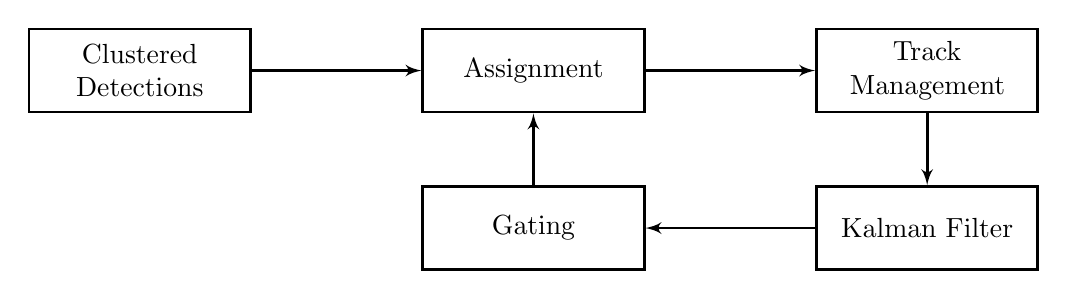
\begin{tikzpicture}[auto,>=latex']
%\draw[gray,very thin] (0,0) grid (15,4); s
   \tikzstyle{block} = [draw, shape=rectangle, minimum height=3em, minimum width=8em, node distance=2cm, line width=1pt]
\tikzstyle{sum} = [draw, shape=circle, node distance=1.5cm, line width=1pt, minimum width=1.25em]
\tikzstyle{branch}=[fill,shape=circle,minimum size=4pt,inner sep=0pt]
%Creating Blocks and Connection Nodes
\node at (3,3) [text width=2 cm,block,align = center] (input) {Clustered  Detections };
\node at (8,3) [block] (h1) {Assignment}; 
\node at (13,3)[text width=2 cm,block,align = center] (h2) {Track \\ Management}; 
\node at (13,1) [block] (h3) {Kalman Filter}; 
\node at (8,1) [block] (h4) {Gating}; 
\begin{scope}[line width = 1pt]
\draw[->] (input) -- (h1);
\draw[->] (h1)--(h2);
\draw[->] (h2) -- (h3); 
\draw[->] (h3)--(h4); 
\draw[->] (h4)--(h1); 

\end{scope}

\end{tikzpicture}
	\caption{MTT-process}
	\label{fig:mtt}
\end{figure} 
Given that usually a constant-velocity model is assumed, a special model needs to be implemented to consider the cases where the target has an (unknown) acceleration. This is issue is handled in \cref{mtt:maneuver}.
\section{State Variable Representation of an LTI System}\label{mtt:state}
A \ac{lti} system can be described by by three variables, input, output and the state variable. In the case of radar, the state can be design to contain several attributes of single targets measured by the radar such as range, range-rate and azimuth angle. Since we desire to determines a target's position and velocity in Cartesian coordinates, the state vector 
\begin{equation}
	\vec{x} = \begin{bmatrix}
	x \\ y \\ v_x \\ v_y
	\end{bmatrix}\\,
\end{equation}
has been chosen. The continuous-time linear system can then be written as
\begin{equation}
	\dot{\vec{x}}(t) = \matrix{A}(t)\vec{x}(t)+ \matrix{B}(t)\vec{u}(t) + \tilde{\vec{v}}(t)\\,
\end{equation}
where $t$ represents time and 
\begin{description}[align=left,labelwidth=1cm]
	\item[$\vec{x}$] is the state vector of dimension $n_x$ and $\dot{\vec{x}}$ its time derivative.
	\item[$\vec{u}$] is the input(or control) vector of dimension $n_u$
	\item[$\tilde{\vec{v}}$] is the process noise
	\item[$\matrix{A}$,$\matrix{B}$] are known matrices of dimensions $n_x\times n_x$ and $n_x\times n_u$
\end{description}
\section{The Kalman Filter}\label{mtt:kalman}
 Different classes of filters (or estimators) have been used for tracking. One of the simplest class of these filters is, for instance, are the so called "Fixed-Coefficient" filters. The most implemented of these are the $\alpha\beta$ and $\alpha\beta\gamma$ trackers [cite]. These filter provide smoothed and predicted data for target position, velocity and in case of the latter, acceleration.  Nonetheless, given the better estimates it provides, the Kalman filter has been implemented primarily for radar-tracking purposes. Additionaly, the Kalman filter presents the following advantages over the Fixed-Coefficient filters.
\begin{enumerate}
	\item The gain coefficients are computed dynamically, i.e. the same filter can be used for targets of different nature
	\item The filter is robust against missed detections
	\item Provides an accurate measure of the covariance matrix, which is relevant for gating and association processes
\end{enumerate}
An overview of the process undertaken by the Kalman filter is presented in \cref{fig:kalman}.
\begin{figure}[h]
	\centering
	
\begin{tikzpicture}
% Reference Grid
\draw[gray,very thin] (0,0) grid (10,4); 

\end{tikzpicture}
	\caption{The Kalman Filter}
	\label{fig:kalman}
\end{figure} 
Before presenting the equations that describe the Kalman filter, the notation is introduced. $\hat{\vec{x}}(n|m)$ represents the estimate during the $n$-th sampling interval using all data up to the $m$-th sampling interval, and $z(n)$ contains the measurements (or detections that have been assigned to the corresponding track) obtained at the $n$-th time-step. 

 \subsection{Estimation in Linear Systems}
 The filtering equation is given by
\begin{equation}
	\vec{x}(n|n) = \vec{x}_s(n) = \vec{x}(n|n-1) + \matrix{W}(n)\vec{v}(n)\\,
\end{equation}
where
\begin{description}
	\item[$\vec{x}_s(n)$] is the smoothed output of the Kalman filter
	\item[$\matrix{W}(n)$] are the dynamically computed filter gains
	\item[$\vec{v}(n)$] is the innovation vector 
\end{description}
The innovation vector contains information about how much the estimate $\vec{x}(n|n-1)$ differs from the newly obtained measurements $y(n)$ and can be written as
\begin{equation}
 \vec{v}(n) = \vec{y}(n) -\matrix{H} \vec{x}(n|n-1)\\,
\end{equation}
where $\matrix{H}$ is called the observation matrix. In our case, the measurement vector has the form 
\begin{equation}
\vec{y}(n) = \begin{bmatrix}
x_m(n) \\ y_m(n) \\ 
\end{bmatrix}\\,
\end{equation}
so that $\vec{v}(n)$ only represent the innovation in the position measurements. Therefore, the observation matrix results in 
\begin{equation}
	\matrix{H} = \begin{bmatrix}
	1 & 1 & 0 & 0 \\
	\end{bmatrix}\\.
\end{equation}
The filter gains are computed at each time step by 
\begin{equation}\label{eq:filtergain}
	\matrix{W}(n+1) = \matrix{P}(n+1|n)\matrix{H}^T\matrix{S}^{-1}(n+1)
\end{equation}
where
\begin{description}
	\item[$\matrix{P}$] represents the predictor covariance matrix and,
	\item[$\matrix{S}$] the measurement prediction covariance.
\end{description}
The state prediction covariance is first calculated recursively by 
\begin{equation}
\matrix{P}(n|n+1) = \Expc\{\vec{x}_s(n+1)\vec{x}^*_s\} = \matrix{A}\matrix{P}(n|n)\matrix{A}^T + \vec{Q}\\,
\end{equation}
where $\vec{Q}$ is the covariance matrix for the input $\vec{u}(n)$. After the filter gains have been calculated by \cref{eq:filtergain}, the state covariance is updated by 
\begin{equation}
	\matrix{P}(n+1|n+1)  = \matrix{P}(n+1|n)-\matrix{W}(n+1)\matrix{S}(n+1)\matrix{W}^T(n+1)\\.
\end{equation}
The innovation covariance, or measurement prediction covariance is given by
\begin{equation}\label{eq:innov}
\matrix{S}(n+1) = \matrix{H}\matrix{P}(n+1|n)\matrix{H}^T +\matrix{R}\\,
\end{equation}
where $\matrix{R}$ is the measurement covariance.
\subsection{Initialization of State Estimators}
After a correct algorithm for multi-target tracking has been implemented, one has to generate an input for the classifiers, which are presented in \cref{ch:cl}. Different characteristics of each of the tracks have been used in literature for classification for various purposes. An overview of the different features that have been used as an input for classifiers is presented in \cref{fe:overview}. The possible selection of features is vast, however given the increase in computation each feature extraction one should select the features resulting in a more reliable classification. This is not straightforward, since the performance of each feature for classification is application-dependent. For each track $j$ at time step $k$ we first generate the $n$-tupel
\begin{equation}
	\breve{v}_j[k] = \left(\hat{\Psi}_{D,1},\hat{\Psi}_{D,2},\hat{\Psi}_{D,3},...,\hat{\Psi}_{D,L}\right) \\,
\end{equation}
containing the normalized range-rated obtained from all clusters contributing to the track.  Other features are stored in $n$-tupels with elements corresponding to the ones in $\breve{v}_j[k]$ as
\begin{equation}
	\breve{a}_j[k] = \left(\hat{a}_{1},\hat{a}_{2},\hat{a}_{3},...,\hat{a}_{L}\right) \\.
\end{equation}

Given that the purpose of this thesis is the classify objects according to their micro-Doppler spectrum, the micro-Doppler effect is explained in detail in \cref{fe:mdoppler}, and some measurement results presenting the micro-Doppler spectrum of pedestrians are given in \cref{fe:results}. 
\section{Gating Techniques}\label{mtt:gating}
Gating is a technique used to eliminate extremely unlikely observation-to-track pairings. A gate is calculated around the output of the Kalman filter (predicted position), and any observation outside of this gate is not further consider for that track. Furthermore if only one observation is found within the gate, then the observation is assigned directly to that track and no further processing is required (see \cref{mtt:assign}). 

\begin{figure}[h]
	\centering
	
\begin{tikzpicture}
% Reference Grid
\draw[gray,very thin] (0,0) grid (10,4); 

\end{tikzpicture}
	\caption{Gating}
	\label{fig:gating}
\end{figure} 


One of the simplest gating techniques is using rectangular gates. A given observation is also said to satisfy the gates of a given track if the all the elements of the innovation vector satisfy 
\begin{equation}
	|\vec{v}(n)| \leq K_G \sigma_r
\end{equation}
where $\sigma_r$ is the residual standard deviation that can be expressed in terms of measurement $\sigma_o^2$ and prediction $\sigma_p^2$
\begin{equation}
	\sigma_r = \sqrt{\sigma_o^2 +\sigma_p^2}\\.
\end{equation}
Note that the values $\sigma_o$ and $\sigma_p$ can be found in the Kalman filter equations as 
\begin{align}
	\sigma_o &= R_{11} & \sigma_p &= P_{11}
\end{align}
The constant $K_G$ can be chosen freely. Usually, a Gaussian error model is assumed to that choosing $K_G = 3$ leads to the probability of a valid observation  satisfying the gating test to be about 99 percent. 
\section{The Assignment Problem}\label{mtt:assign}
In a dense target environment, the gating technique is not sufficient enough to discriminate between detections. Thus a further assignment logic has to be implemented. Conflicts can occur for instance, when a detection satisfies the gating of different tracks, or when a track was multiple detections within its gate. This problem is called the assignment problem. 

There are basically two types of solutions. The  \ac{nn}-approach (\cref{mtt:nn}) and the "all-neighbors" approach (\cref{mtt:pda} and \cref{mtt:jpda}). The first step of all solutions, however, is the same. First, an assignment matrix is built. For this, the norm of the innovation vector that would result if track $i$ and detection $j$ would be assigned is defined as 

\begin{equation}
d_{ij}^2 \triangleq \vec{v}_{ij}(n)^T \matrix{S}_i^{-1}(n)\vec{v}_{ij}(n)\\,
\end{equation}
where $\matrix{S}_i(n)$ is the residual covariance matrix defined in \cref{eq:innov}. Furthermore, it is assumed that the residual has a Gaussian distribution
\begin{equation}
	g_{ij} =\frac{\exp(-\frac{d_{ij}^2}{2})}{(2\pi)^{M/2}\sqrt{|\matrix{S}_i|}}\\,
\end{equation}
where $M$ is the measurement dimension and $|\matrix{S}_i|$ the determinant of $\matrix{S}_i$.
\begin{figure}[h]
	\centering
	
\begin{tikzpicture}
% Reference Grid
\draw[gray,very thin] (0,0) grid (10,4); 

\end{tikzpicture}
	\caption{Example of conflict situations for assignment}
	\label{fig:assign}
\end{figure} 

The basic goal is to make assignment decisions based on the maximization of $g_{ij}$, which is equivalent to minimizing the quantity 
\begin{equation}
	d_{Gij}^2 = d_{ij}^2 + \ln |\matrix{S}_i|\\,
\end{equation}
which will be used as distance function for use in the assignment problem.


\subsection{NN-approach}\label{mtt:nn}
For the \ac{nn} approach, first an assignment matrix as the one depicted in \cref{fig:assignM} is built. Observations that are know within the gate of a certain track, will be identified as $X$. Otherwise, the distance function of of the corresponding observation and track is calculated. 

\begin{figure}[h]
	\centering
	
\begin{tikzpicture}
% Reference Grid
\draw[gray,very thin] (0,0) grid (10,4); 

\end{tikzpicture}
	\caption{Assignment matrix example}
	\label{fig:assignM}
\end{figure} 

There are different ways to solve the assignment problem from the assignment matrix following a \ac{nn}-approach.Two suboptimal solutions are presented and (LATER: OPTIMAL SOLUTION).

Suboptimal Solution one:
\begin{enumerate}
	\item Observations that are considered for singly-validated tracks will not be considered for mutiply-validated tracks. 
	\item Observations that are in multiple tracks will not be considered for tracks that contain single-validated observations
	\item Repeat 1. and 2. until the assignment matrix is not changed anymore 
	\item For the remaining tracks with multiple observations, select the observation with minimum distance 
	\item For the remaining observations that validate with various tracks, assign to th track with the minimum distance
\end{enumerate}

Suboptimal Solution two:
\begin{enumerate}
    \item Search the matrix for the minimum distance observation-to-track pair and assign it
    \item  Remove the assigned pair from the matrix and repeat 1. until all possible assignments have been made. 
\end{enumerate}
\subsection{PDA-approach}\label{mtt:pda}
\subsection{JPDA-approach}\label{mtt:jpda}
\section{Track Life Stages}\label{mtt:management}
NOTE: For now very simple methods for track management have been implemented:

Track Initiaiton: Any detection not assigned
Track Confirmation: If a tentative track has at least 3 detections for 5 time steps
Track Deletion: After 10 consecuitive missed detections

\begin{figure}[h!]
	\centering
	
\begin{tikzpicture}
% Reference Grid
\draw[gray,very thin] (0,0) grid (10,4); 

\end{tikzpicture}
	\caption{Density-reachable example}
\end{figure} 

\subsection{Track Confirmation}
\subsection{Track Deletion}
\section{Maneuver Detection and Adaptive Filtering}\label{mtt:maneuver}
\chapter{Micro-Doppler Signatures}
\chapter{Classification}
\chapter{Results}
\chapter{Summary and Outlook}
\begin{appendices}
\chapter{Symbols and Constants}
\section*{General}
\begin{longtable}{ p{.20\textwidth}  p{.80\textwidth} } 
% Lateinische Buchstaben
$ \oint $ & Integration over a closed curve \\
\addlinespace[15pt]
\end{longtable}
\section*{Latin alphabet}	
\begin{longtable}{ p{.20\textwidth}  p{.80\textwidth} } 
% Lateinische Buchstaben
$R$ & Range \\
$R_u$ & Unambiguous Range \\
\addlinespace[15pt]
\end{longtable}
\section*{Greek alphabet}	
\begin{longtable}{ p{.20\textwidth}  p{.80\textwidth} } 

%Griechische Buchstaben
$ \Delta T $ & Delay\\
\addlinespace[15pt]
\end{longtable}
\section*{Constants}	
\begin{longtable}{ p{.10\textwidth}  p{.075\textwidth}  p{.80\textwidth}} 
% Lateinische Buchstaben
$ c_0 $ & $=$ & \unit[299729458]{m/s} \\
\addlinespace[15pt]
\end{longtable}
\chapter{Mathematical Formulas}


\end{appendices}
\newpage

\bibliography{misreferencias}


\newpage
\end{document}
